\subsection{Problema 1 - \texorpdfstring{$M$}{M}-QAM}

Considere a modulação $M$-QAM, em que o sinal em banda base é dado por:
$$s_m(t) = ( A_m^{(\text{real})} + j A_m^{(\text{imag})}) g(t) ,$$
em que $g(t)$ é um pulso transmitido, $A_m^{(\text{real})}$ e $A_m^{(\text{imag})}$ são amplitudes da parte real e imaginária da forma de onda transmitida, respectivamente.

% Considere $\int_{-\inf}^{\inf} |g(t)|^2 \,dt = \mathcal{E}_{g} = 1$, isto é, o pulto $g(t)$ possui energia unitária. Suponha a transmissão de uma sequência de símbolo $\{s_{m}\}$ de tamanho $L = 26400 \text{bits}$
% \begin{enumerate}
%     \item A energia média $\mathcal{E}_{m}$ de cada constelação;
%     \item A distância mínima $d_{min}$ entre dois símbolos;
%     \item O modulador (mapeamento bit-símbolo) usando a codificação de Gray;
%     \item O demodulador (mapeamento símbolo-bit).
% \end{enumerate}

% -------------------------------------------------------------------

\subsubsection{Energia da Constelação} 

O desenvolvimento é citado em~\cite{Proakis, Cecilio}.

$$ \mathcal{E}_{media} = \frac{M-1}{3} \mathcal{E}_g$$

$$ \mathcal{E}_{media(bit)} = \frac{M-1}{3\log_2 M} \mathcal{E}_g $$
% -------------------------------------------------------------------
\subsubsection{Distância Mínima entre Símbolos}

Como calcular os coeficiente para constelação $M$-QAM retangular, onde $\sqrt{M}$ assume valores inteiros. Os coeficientes em quadratura $a_i$ e $b_i$ são obtidos através da equação: $\{ (2i -\sqrt{M} - 1)d \}_{i=1}^{\sqrt{M}} $ 

A distância eucliadiana entre os sinais na modulação QAM é
$$ d_{mn} = \sqrt{|| s_m - s_n||^2}$$ 
$$ = \sqrt{\frac{\mathcal{E}_g}{2}[(A_{mi} - A_{ni})^2 + (A_{mq} - A_{nq})^2]}$$

$$\sqrt{\frac{3 \mathcal{E}_{media}}{2(M-1)}} $$

\begin{table}[!ht]
    \centering
    \begin{tabular}{|c|c|c|c|}
    \hline
    $M$-QAM & $\mathcal{E}_{media}$ & $\mathcal{E}_{media(bit)}$ & $d$ \\ \hline
    & &  &  \\ 
    $M$ & $\frac{M-1}{3} \mathcal{E}_g$ & $ \frac{M-1}{3\log_2 M} \mathcal{E}_g$ & $\sqrt{\frac{3 \mathcal{E}_{media}}{2(M-1)}} $ \\ 
    & &  &  \\ \hline
    & &  &  \\ 
    $4$     & 1 & $1.67\times 10^{-1}$ & $\frac{\sqrt{2}}{2}$ \\ 
    & &  &  \\ \hline
    & &  &  \\ 
    $16$    & 5 & $4.67\times 10^{-1}$ & $\frac{\sqrt{2}}{2}$ \\ 
    & &  &  \\ \hline
    & &  &  \\ 
    $64$    & 21 & $1.17\times 10^{0}$ & $\frac{\sqrt{2}}{2}$ \\
    & &  &  \\ \hline
    \end{tabular}
    \caption{Informações gerais calculadas para a modulação $M$-QAM.}
    \label{tab:Resume_QAM}
\end{table}

\clearpage

\subsubsection{Modulador (Codificação de Gray)}

\begin{figure}[!ht]
    \centering
    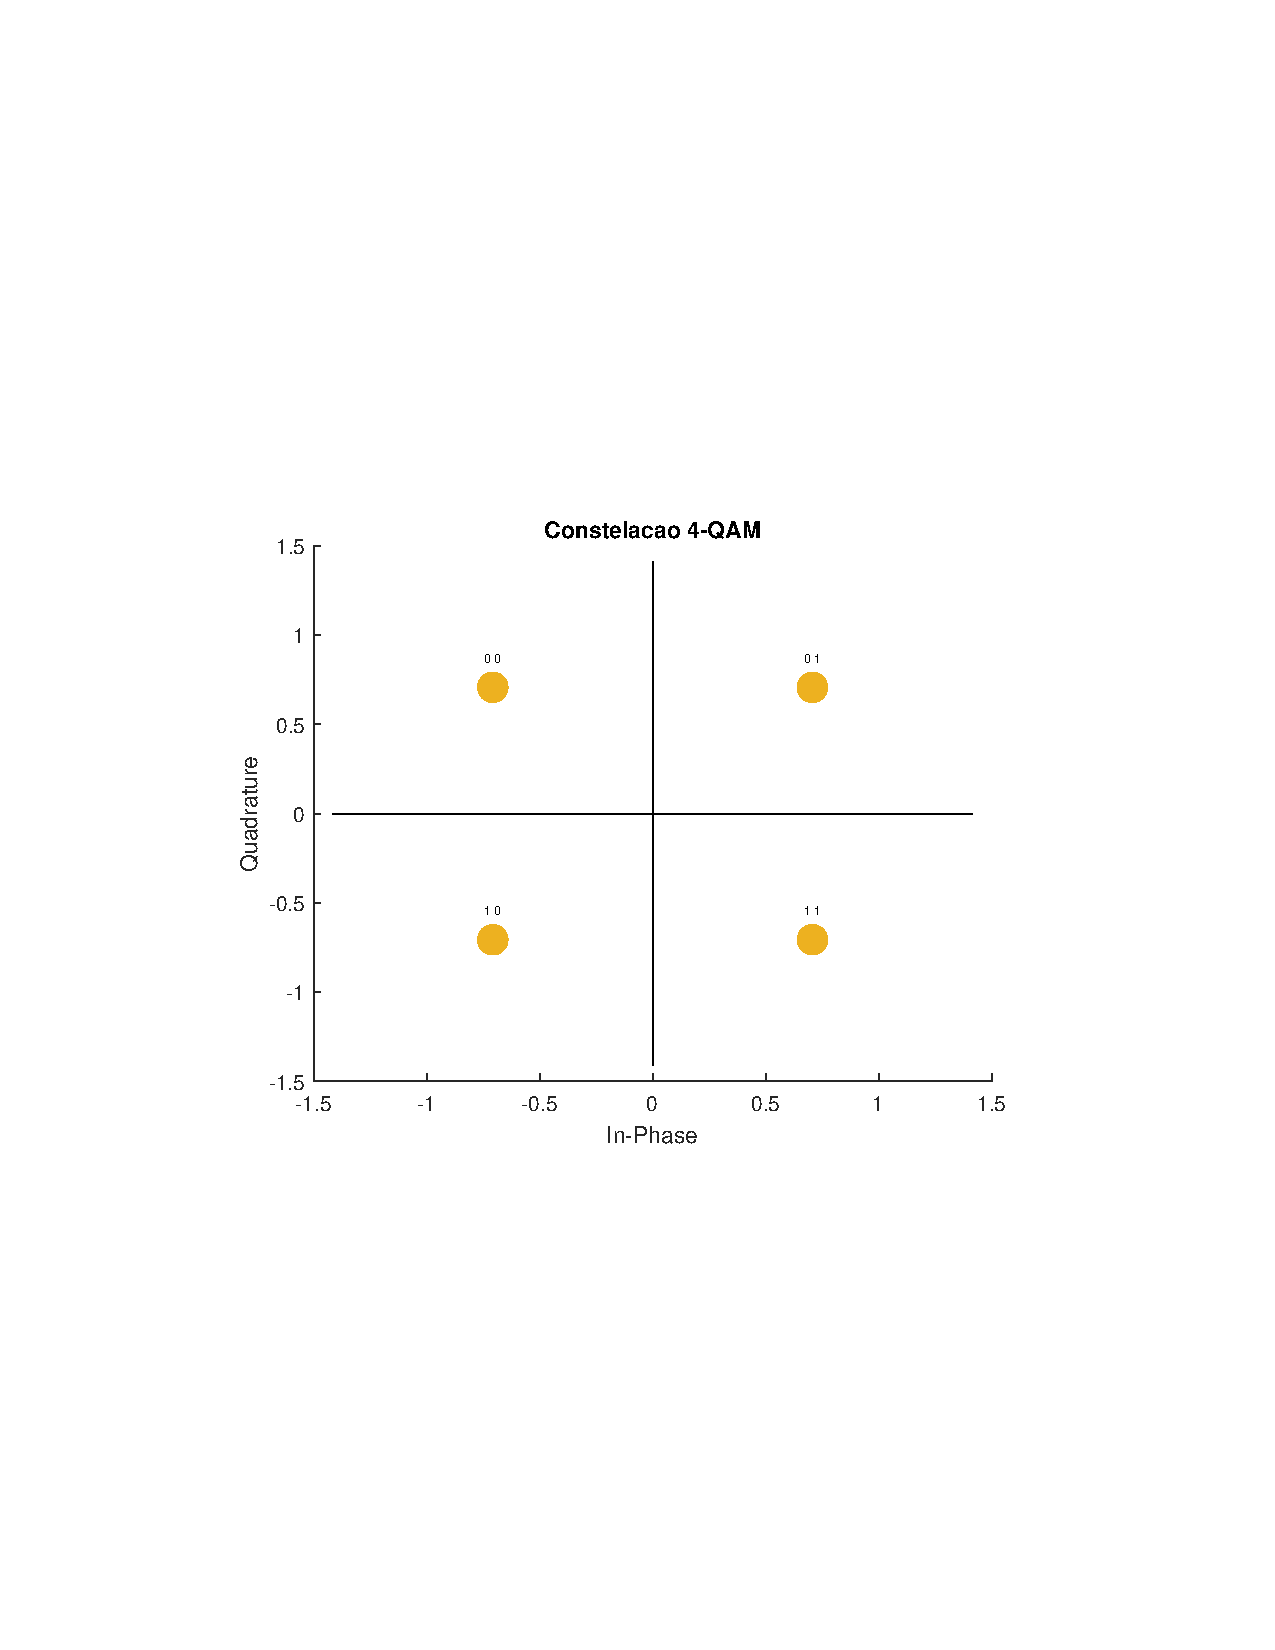
\includegraphics[width=1.0\textwidth,clip=true,trim={1.5cm 8.5cm 1.8cm 8.3cm}]{C:/Users/lukin/Documents/GitHub/Courses-HWs/Sistemas de Comunicacoes Digitais/matlab/problema1/fig/4_QAM_plot.pdf}
    \caption{Exemplo de 4-QAM plot.}
    \label{fig:4_QAM_plot}
\end{figure}

\begin{table}[!ht]
    \centering
    \begin{tabular}{|c|c|c|c|}
    \hline
    Decimal & Binário & Gray & Decimal \\ \hline
    0 & 00 & 00 & 0\\ \hline
    1 & 01 & 01 & 1\\ \hline
    2 & 10 & 11 & 3\\ \hline
    3 & 11 & 10 & 2\\ \hline
    \end{tabular}
    \caption{Tabela de tradução de binário para Gray com 2 bits.}
    \label{tab:Alfabeto_Gray}
\end{table}

Algoritmo para obter o código de Gray~\ref{alg:Gray}

% global change
\SetKwInput{KwData}{Entrada}
\SetKwInput{KwResult}{Saída}

\begin{algorithm}[!ht]
    \SetAlgoLined
    \KwData{Sequência de Bits $(b)$ - MSB}
    \KwResult{Sequencia em Código Gray $(g)$ - LSB}
    $n = 0$\;
    $K = \text{length}(b)$\;
    \While{$K > n$}{
        \eIf{$K==n$}{
            $g_{(K-n)} = b_{(K-n)}$ \;
            }{
            $g_{(K-n)} = b_{(K-n+1)} \otimes b_{(K-n)}$\;
        }
        $n=n+1$;\;
     }
     $g = flip(g)$\;
     \caption{Codificação de Gray}
     \label{alg:Gray}
\end{algorithm}

\clearpage



\begin{figure}[!ht]
    \centering
    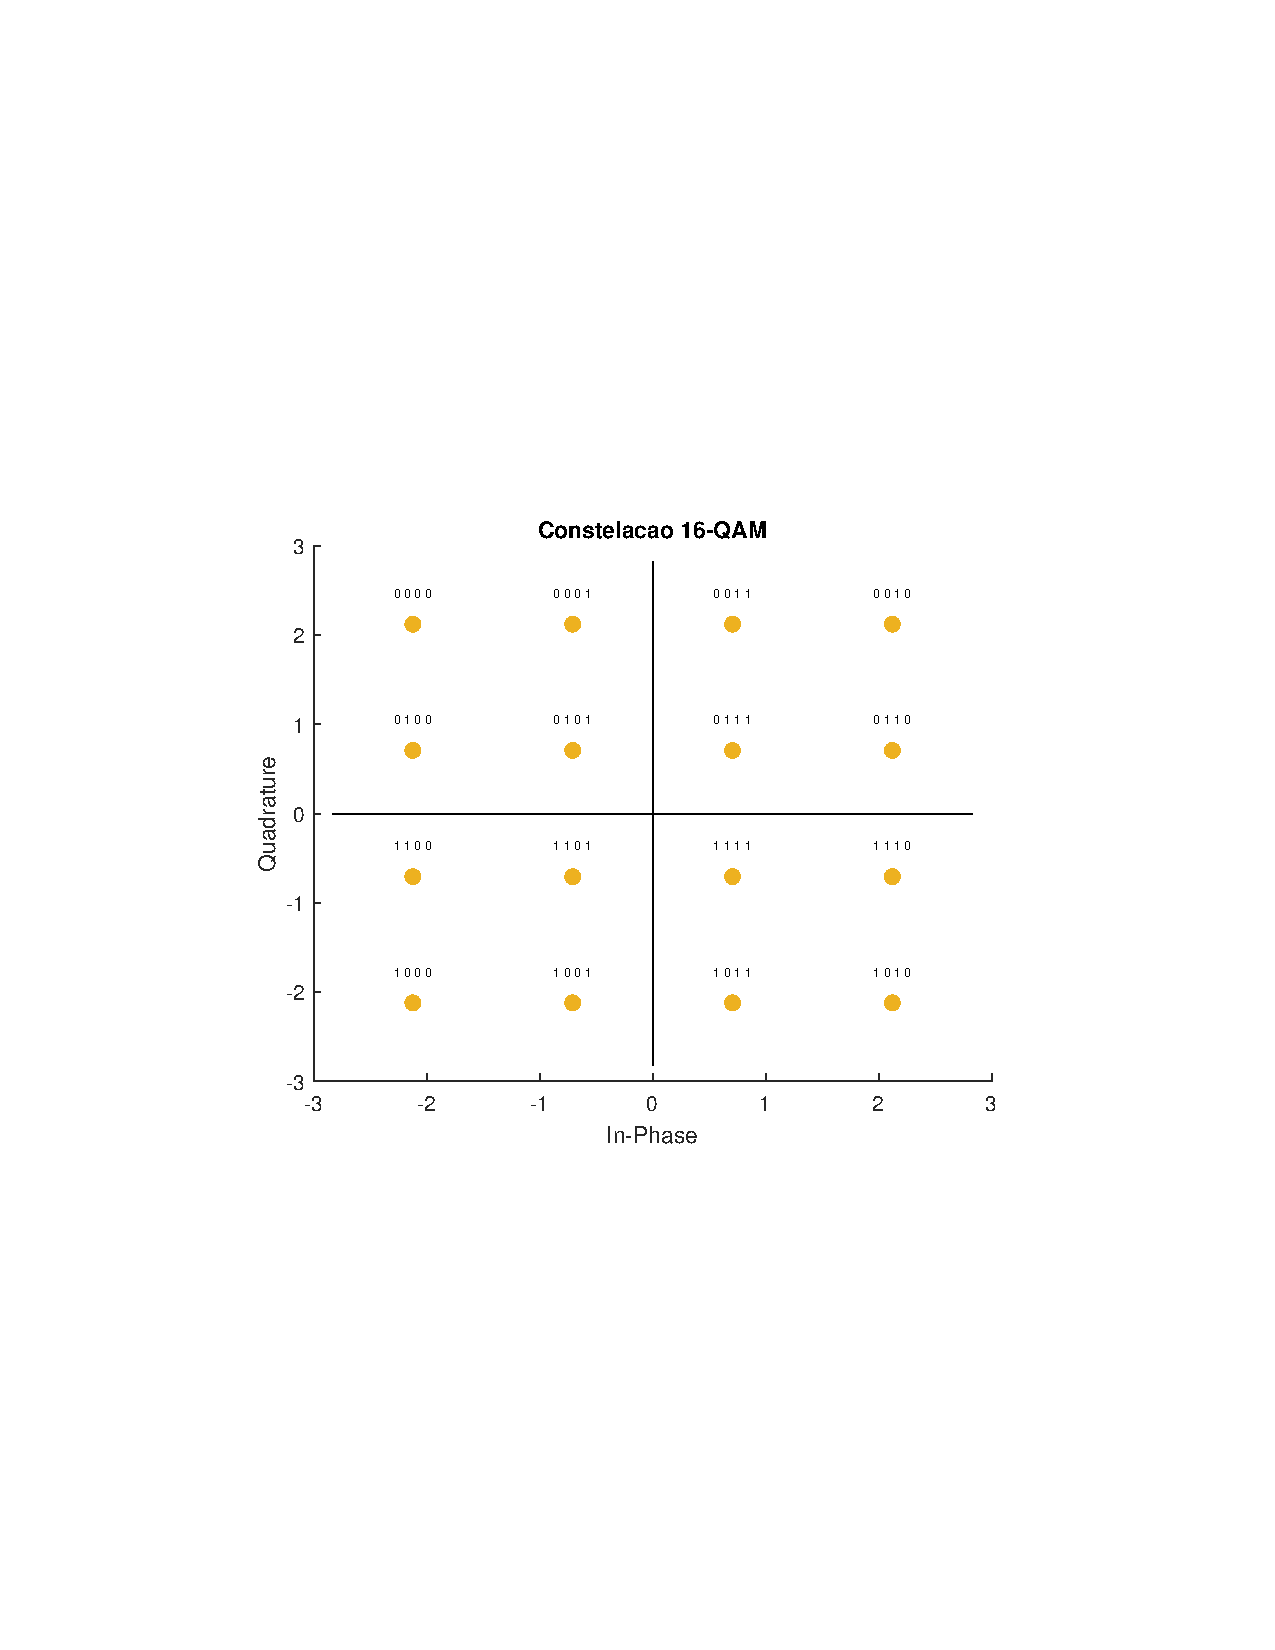
\includegraphics[width=1.0\textwidth,clip=true,trim={1.5cm 8.5cm 1.8cm 8.3cm}]{C:/Users/lukin/Documents/GitHub/Courses-HWs/Sistemas de Comunicacoes Digitais/matlab/problema1/fig/16_QAM_plot.pdf}
    \caption{Exemplo de 16-QAM plot.}
    \label{fig:16_QAM_plot}
\end{figure}

\begin{figure}[!ht]
    \centering
    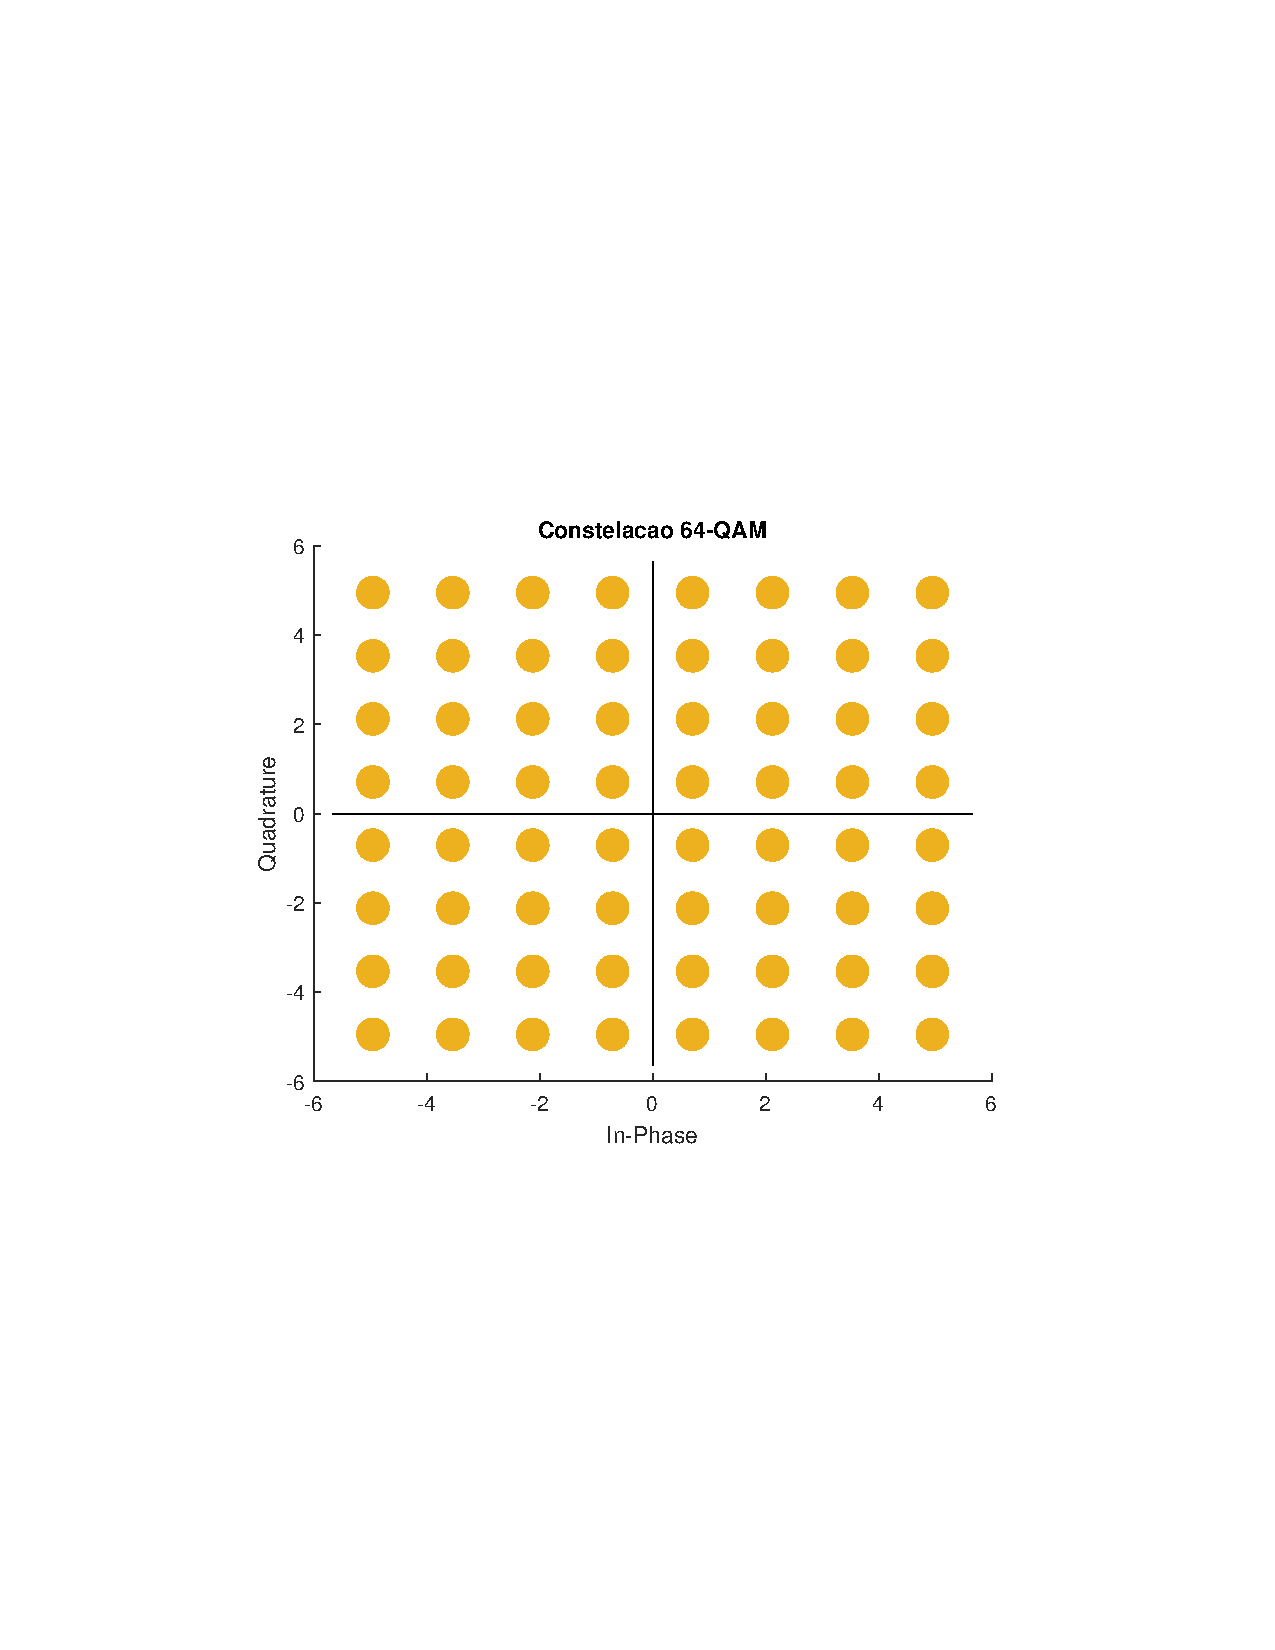
\includegraphics[width=1.0\textwidth,clip=true,trim={1.5cm 8.5cm 1.8cm 8.3cm}]{C:/Users/lukin/Documents/GitHub/Courses-HWs/Sistemas de Comunicacoes Digitais/matlab/problema1/fig/64_QAM_plot.pdf}
    \caption{Exemplo de 64-QAM plot.}
    \label{fig:64_QAM_plot}
\end{figure}

\clearpage

% -------------------------------------------------------------------
\subsubsection{Demodulador}

Considerando $\mathcal{E}_g = \int_{-\infty}^{\infty} |g(t)|^2 \,dt = 1$, a energia média da constelação pode ser calculada por $\epsilon$



%%
% Please add the following required packages to your document preamble:
